\chapter{Fudamentação Teórica}
\label{fundamentacao}

{\color{red} Introdução...}

\section{Metodologias Ágeis}
\label{fundamentacao:ageis}

{\color{red} Metodologias Ágeis...}

\subsection{Fatores-Chave do Trabalho em Equipe}
\label{fundamentacao:ageis:fatores}

Como forma de elencar os fatores que influenciam o TE de equipes ágeis, foi realizada uma Revisão Literária, adotando alguns aspectos de Revisões Sistemáticas, para garantir uma maior quantidade de trabalhos relevantes encontrados. Apesar de não seguir o protocolo necessário para realizar uma Revisão Sistemática em Engenharia de \textit{Software} \cite{kitchenhan}, adotou-se nessa Revisão Literária as duas fases essenciais de Revisões Sistemáticas para selecionar estudos relevantes. A primeira fase é de Seleção de Estudos, onde a relevância dos trabalhos para o contexto desta pesquisa foi avaliada com base nos títulos, \textit{abstracts} e palavras-chave desses trabalhos. Em seguida, com base nessas propriedades dos trabalhos, os estudos irrelevantes e duplicados são descartados. Depois disso, ocorre a fase de Extração dos Estudos, ou Avaliação da Qualidade dos Trabalhos. Nessa fase, os trabalhos considerados relevantes após a fase de Seleção de Estudos foram avaliados com base em suas introduções e conclusões, além de suas respectivas qualidades. Assim, são descartados mais alguns trabalhos. Finalmente, as informações relevantes para esta pesquisa foram extraídas dos trabalhos remanescentes.

Para realizar esse processo, os motores de busca selecionados para servir de fonte de trabalhos foram: \textit{ACM}\footnote{\url{http://dl.acm.org/}}, \textit{IEEE}\footnote{\url{http://ieeexplore.ieee.org/Xplore/home.jsp}}, \textit{Scopus}\footnote{\url{http://www.scopus.com/}}, \textit{Science Direct}\footnote{\url{http://www.sciencedirect.com/}} e \textit{Google Scholar}\footnote{\url{https://scholar.google.com.br/}}. Em seguida, foram definidas as \textit{strings} de busca para cada um desses motores. Além disso, foi utilizada a ferramenta \textit{StArt}\footnote{\url{http://lapes.dc.ufscar.br/tools/start_tool}} para auxiliar a gerência das informações referentes aos trabalhos encontrados.

Ao final dessa Revisão Literária, foram identificados 20 fatores que influenciam a qualidade do TE em equipes ágeis. Esses fatores estão descritos na Tabela \ref{fundamentacao:ageis:fatores:tabela}.


A \textit{Comparative Agility}\footnote{\url{https://comparativeagility.com/}} é uma ferramenta web quer permite avaliar o quão ágil uma organização é em relação à outras. De acordo com o site, essa ferramenta é considerada a mais abrangente em relação à avaliação ágil na indústria. Essa avaliação é feita com base em um \textit{survey} organizado em sete dimensões e trinta e duas características. Uma das dimensões consideradas nessa ferramenta é o \textit{Trabalho em Equipe}. Essa dimensão é dividida em três características (i.e., Composição da Equipe, Gerenciamento e Comunicação). Para cada uma dessas características, há perguntas relacionadas a fatores que influenciam essas características. A Figura \ref{fundamentacao:ageis:fatores:comparativeagility} representa o relacionamento entre a dimensão \textit{Trabalho em Equipe}, suas características e os aspectos que contribuem para a boa qualidade dessas características.

\begin{figure}[ht!]
\begin{center}
        \fbox{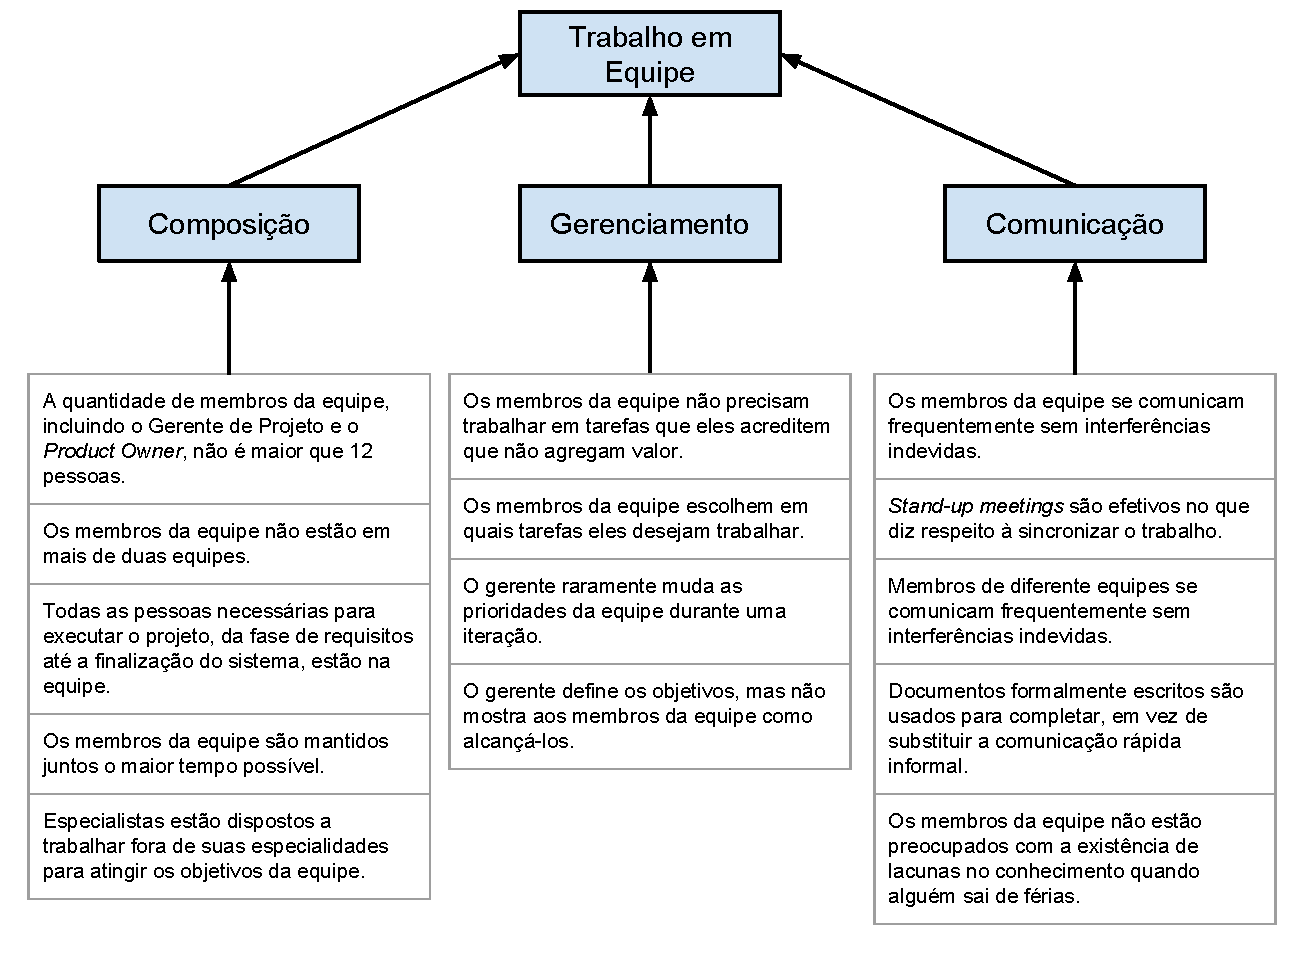
\includegraphics[scale=0.67]{figs/comparativeAgility_teamwork.pdf}}
    \end{center}
    \caption{Representação do Trabalho em Equipe na Ferramenta \textit{Comparative Agility}.}
    \label{fundamentacao:ageis:fatores:comparativeagility}
\end{figure}

\section{Redes Bayesianas}
\label{fundamentacao:redes}

{\color{red} Redes Bayesianas...}

\subsection{Construção de Redes Bayesianas}
\label{fundamentacao:redes:construcao}

{\color{red} Construção...}

\subsection{Nós Ranqueados}
\label{fundamentacao:nos}

{\color{red} Nós Ranqueados...}
